
\section{Introduction to Intelligent Industrial Automation Systems}

The landscape of industrial automation has undergone a profound transformation in recent decades, evolving from rigid, centralized control systems to flexible, distributed architectures that can adapt to dynamic production requirements. This evolution has been driven by the increasing complexity of manufacturing processes, the demand for mass customization, and the need for sustainable, energy-efficient operations. The integration of emerging technologies such as blockchain, artificial intelligence, and multi-agent systems has opened new possibilities for creating intelligent, self-adapting industrial control systems that can operate autonomously while maintaining high levels of reliability and efficiency.

The IEC 61499 standard has emerged as a cornerstone technology in this transformation, providing a framework for designing distributed control systems that emphasize modularity, interoperability, and portability. Unlike its predecessor IEC 61131-3, which focused on centralized programmable logic controllers, IEC 61499 facilitates the development of flexible and reusable control systems that can adapt to changing process requirements without extensive reprogramming. This standard supports event-driven control activities, enabling more responsive and efficient systems particularly suitable for complex, distributed industrial environments.

However, the implementation of truly intelligent industrial automation systems faces several critical challenges. First, the vast amount of data generated by modern control systems often overwhelms traditional analysis methods, making it difficult to extract actionable insights in real-time. Second, the need for product traceability and process verification in flexible manufacturing environments requires robust, tamper-proof recording mechanisms. Third, the complexity of system testing and validation, especially for safety-critical applications, demands automated approaches that can handle the increasing sophistication of control logic.

This chapter presents three complementary approaches to addressing these challenges: blockchain-enabled product traceability, large language model-based human-machine interaction, and knowledge-driven AI agents for planning and testing. Each approach contributes to different aspects of intelligent industrial automation, and their integration represents a comprehensive solution for the next generation of manufacturing systems.

\section{Blockchain-Enabled Product Traceability and Verification}

The integration of blockchain technology into industrial control systems represents a paradigm shift in how manufacturing processes are recorded, verified, and validated. Blockchain's inherent characteristics of decentralization, immutability, and transparency make it particularly well-suited for addressing the challenges of product traceability in flexible and reconfigurable automation systems.

\subsection{Blockchain Technology in Industrial Control Systems}

Blockchain technology offers a decentralized and immutable ledger for securely recording each step of the production process. In industrial control systems, this capability addresses the critical need for transparent traceability of products from raw materials to finished goods, ensuring authenticity and accountability throughout the manufacturing process. The Ethereum blockchain, with its smart contract functionality, provides a particularly powerful platform for industrial applications by enabling the creation of self-executing contracts with predefined rules and conditions.

Smart contracts automate predefined processes, ensuring consistency and reliability while providing transparency and immutability that enables stakeholders to verify and trace process executions. These contracts incorporate validation mechanisms to ensure adherence to criteria or standards, enhancing reliability and compliance. The Ethereum Virtual Machine (EVM) serves as the runtime environment for executing these smart contracts, allowing for decentralized processing of code and transactions on the network.

\begin{figure}[h]
    \centering
    \includegraphics[width=0.8\textwidth]{MX_Papers/Paper11/images/Architecture.pdf}
    \caption{Architectural design for blockchain-powered product traceability in multi-agent systems, showing the integration of user agents, processing agents, execution agents, and verifying agents with blockchain technology}
    \label{fig:blockchain_architecture}
\end{figure}

\subsection{Multi-Agent Systems for Process Verification}

The combination of blockchain technology with multi-agent systems creates a powerful framework for process verification and validation. Multi-agent systems, with their adaptable and reconfigurable structure, facilitate agile responses to changes in operational needs, enabling seamless adjustments in manufacturing processes. These systems exhibit considerable advancements within Industry 4.0 initiatives by effectively addressing intricate challenges inherent in industrial control systems.

The proposed architectural design for blockchain-powered product traceability employs various types of software agents: user agents, processing agents, execution agents, and verifying agents. User agents manage order processes and assess compatibility with system capabilities. Processing agents craft process recipes and oversee execution, formulating proposals and sharing them with registered agents possessing equivalent capabilities. Execution agents review proposals and execute skills using IEC 61499 function blocks, while verifying agents ensure that actual process recipes have been followed correctly.

The workflow begins when a user initiates product creation by executing a transaction on the blockchain. Software agents then accept the order request and generate a process recipe tailored to the user's specifications. The agents utilize IEC 61499 function blocks to execute tasks according to the process recipe, with metadata including process description, status, timestamp, and additional information recorded using smart contracts at each step. Finally, verification of process sequences within the customized product's recipe is conducted by cross-referencing the metadata associated with the product on the blockchain.

\subsection{Smart Contracts for Automated Compliance}

Smart contracts provide a secure and transparent way to store data on the blockchain, ensuring immutability and tamper-proof recording of events. In flexible production systems, smart contracts enhance traceability by creating an auditable record of each step in the production process. With data securely recorded on the blockchain, stakeholders can trace the origin and journey of products and verify authenticity, promoting trust among participants and enabling faster identification and resolution of issues.

The implementation of smart contracts in industrial control systems addresses several key challenges. First, it provides real-time verification of product adherence to correct process orders, enabling the prompt identification and removal of defective products. Second, it offers customers transparent access to production process information through block verification, enhancing trust and accountability. Third, it creates an immutable record of all process executions, facilitating compliance with regulatory requirements and quality standards.

The use of InterPlanetary File System (IPFS) for off-chain storage of large files, such as video or image records of product executions, further enhances the system's capabilities. This approach avoids direct blockchain storage by generating unique Content IDs (CIDs) for each file and placing the actual data on a network of distributed nodes. This strategy alleviates the burden on individual blockchain nodes while maintaining the integrity and immutability of the data through the use of CIDs in blockchain transactions or smart contracts.

\section{Large Language Models for Enhanced Human-Machine Interaction}

The integration of large language models (LLMs) into industrial control systems represents a significant advancement in human-machine interaction, enabling operators to interact with complex systems using natural language. This capability addresses the challenge of data retrieval and analysis in industrial environments, where the vast amount of generated data is often complex and cumbersome to analyze due to its sheer volume and variety.

\subsection{Conversational AI in Industrial Environments}

LLMs excel in natural language understanding (NLU) and natural language generation (NLG), making them highly effective for tasks involving language translation, summarization, question answering, and complex reasoning. The integration of LLMs into industrial control systems significantly enhances human-machine interfaces (HMIs), making them more intuitive and accessible through conversational AI. Operators can interact with machines using natural language to perform tasks such as querying system status, issuing commands, or troubleshooting, which reduces technical barriers and improves user experience.

The application of LLMs in industrial settings extends beyond simple query processing to include sophisticated analysis and visualization of intricate datasets. These models can revolutionize documentation and reporting by automating the creation of detailed operational records and incident reports, improving the accuracy and timeliness of critical data for compliance and operational reviews. Additionally, LLMs offer predictive maintenance capabilities by analyzing historical and real-time data to predict equipment failures, thus minimizing downtime and extending the useful life of equipment.

\begin{figure}[h]
    \centering
    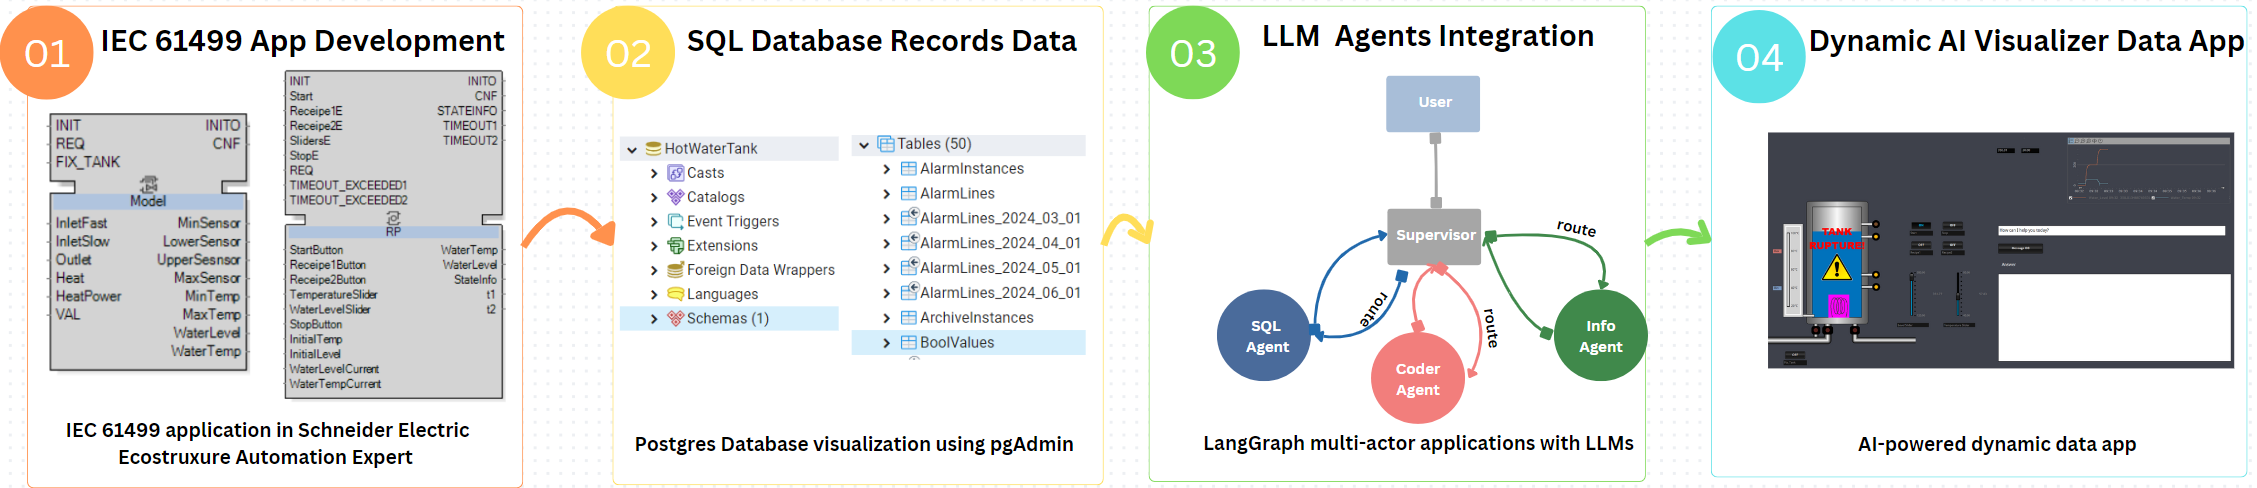
\includegraphics[width=0.9\textwidth]{MX_Papers/Paper12/images/workflow.PNG}
    \caption{Workflow for developing intelligent multi-actor applications with LLMs for data analysis and visualization of IEC 61499-based control systems, showing the four-stage process from application construction to HMI integration}
    \label{fig:llm_workflow}
\end{figure}

\subsection{Multi-Actor LLM Frameworks}

The development of multi-actor LLM frameworks represents a sophisticated approach to leveraging artificial intelligence in industrial control systems. These frameworks utilize specialized LLM actors that interact through graph-based multi-actor architectures, addressing various aspects of IEC 61499 control systems including PLC code analysis, SQL query execution, and data visualization.

LangChain and LangGraph serve as foundational technologies for building these multi-actor systems. LangChain is an advanced software library designed to enhance the functionality of LLMs by facilitating the integration of external knowledge and reasoning capabilities. This framework supports the seamless combination of natural language processing tasks with data retrieval, offering a structured approach to managing workflows that incorporate external APIs, databases, and custom logic.

LangGraph, on the other hand, is an innovative framework designed to increase the capabilities of LLMs by integrating them with graph-based data structures. This integration allows LLMs to leverage structured information in the form of graphs, enhancing their ability to understand relationships and dependencies between various entities and concepts. By utilizing LangGraph, LLMs can access and manipulate knowledge graphs, which store information in nodes and edges representing entities and their interconnections, respectively.

\subsection{Natural Language Processing for Data Analysis}

The application of natural language processing in industrial data analysis addresses the challenge of extracting actionable insights from complex datasets. Traditional methods, which frequently rely on SQL queries for data retrieval, can be inefficient and time-consuming, requiring specialized skills to formulate and execute. The complexity of these queries often hinders the ability to quickly extract actionable insights from the data, which is critical to timely decision-making and operational adjustments.

LLM-based approaches to data analysis include several key components. First, Retrieval Augmented Generation (RAG) techniques enhance the knowledge base of LLMs with additional data, enabling them to deliberate on private data or information introduced after a model's training cut-off. In the context of industrial control systems, the use of IEC 61499 XML files as supplementary data for LLMs enhances their understanding of system intricacies, enabling detailed insights about system components, devices, applications, and function blocks.

Second, SQL agents provide sophisticated methods for constructing query and answer chains over SQL databases, allowing users to pose questions about data and receive answers in natural language. These agents offer dynamic interaction with SQL databases compared to standard query chains, enabling them to answer queries based not only on database content but also on database schema descriptions. The agents are equipped to handle errors effectively by catching tracebacks from failed query executions and regenerating queries correctly.

Third, visualization agents enhance LLM functionality through tool integration for dynamic data visualization. These agents can utilize values extracted from databases to plot graphs, demonstrating advanced applications of chains and agents that can invoke tools ranging from APIs and functions to databases. The critical aspect of integrating models with tools lies in the effective prompting of the model and accurate parsing of its responses, ensuring the selection of appropriate tools and correct input for these tools.

\section{Knowledge-Driven AI Agents for Planning and Testing}

The development of knowledge-driven AI agents represents a significant advancement in industrial automation, enabling intelligent planning, validation, and testing of control systems through semantic reasoning and automated decision-making. These agents address the critical challenges of generating energy- and cost-efficient operational plans and automating the testing and validation of complex control systems.

\subsection{Semantic Reasoning in Industrial Automation}

Knowledge-driven AI agents leverage semantic reasoning to interpret natural language instructions, infer control system requirements, and autonomously generate optimized sequences of machine skills to fulfill tasks. The architecture of these systems typically consists of a hierarchy of AI agents orchestrated by a triage agent, which coordinates planning, validating, and testing agents. All agents share access to a centralized knowledge graph that encodes the system's configuration, available services (skills), execution costs, rules, and dependencies.

The planning agent generates optimized skill sequences to fulfill user-defined objectives by querying the knowledge graph using semantic functions such as \textit{getPhysicalConfiguration()}, \textit{getSkillInfo()}, and \textit{getSensorInfo()} to collect relevant domain knowledge. To minimize noise in the knowledge graph, the planning agent leverages targeted queries via function calling to extract only relevant and context-specific information, effectively filtering out irrelevant or conflicting data. It then reasons over the retrieved data, considering operational constraints such as energy usage, time, and dependency rules, and constructs a plan accordingly.

\begin{figure}[h]
    \centering
    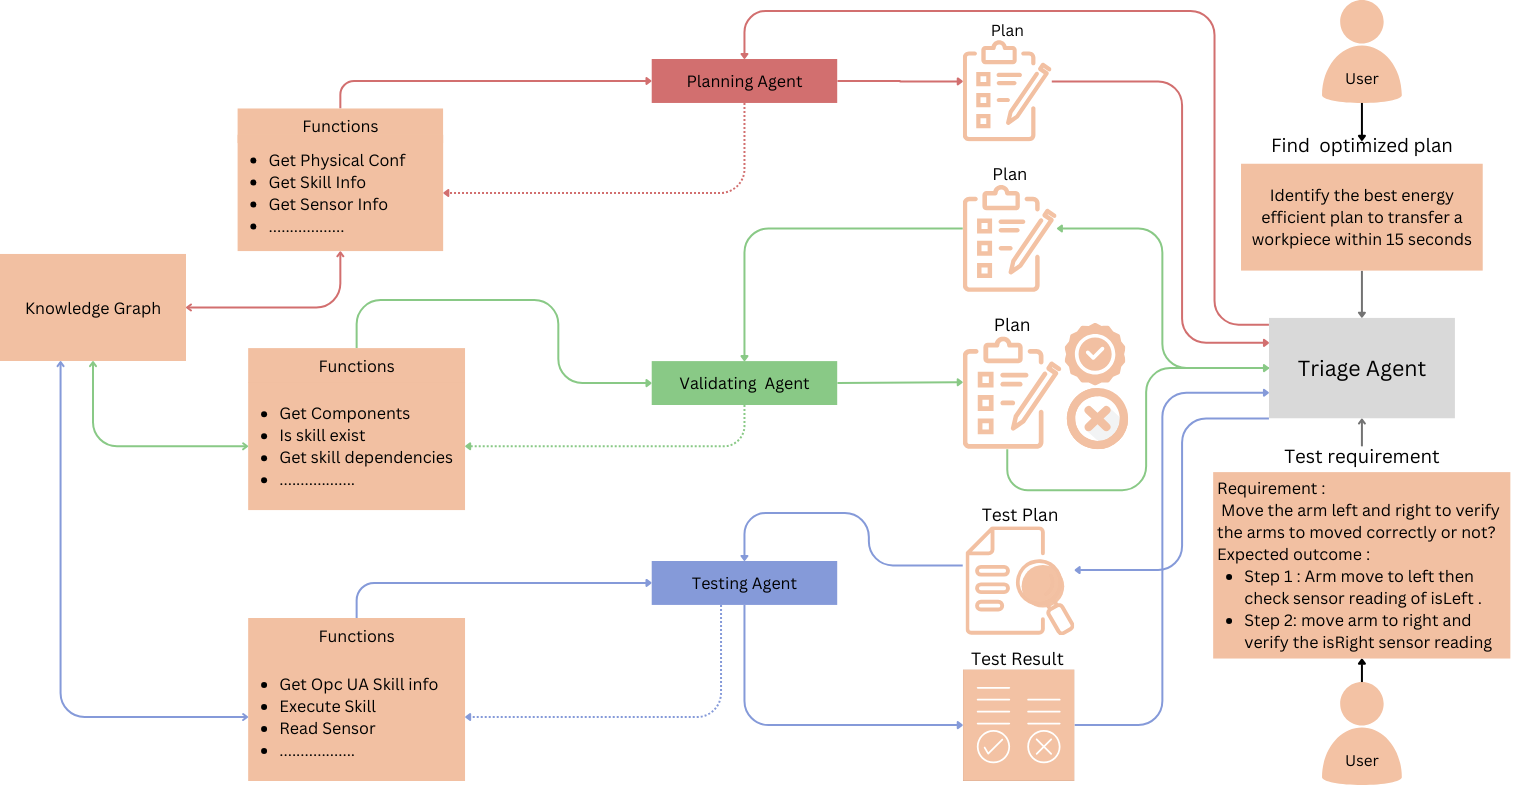
\includegraphics[width=0.9\textwidth]{MX_Papers/Paper13/images/arch.png}
    \caption{Multi-agent system architecture for planning, validation, and testing of industrial control systems, showing the coordination between triage, planning, validating, and testing agents}
    \label{fig:ai_agent_architecture}
\end{figure}

The validating agent is responsible for verifying whether proposed plans adhere to operational rules and resource constraints defined in the knowledge graph. It checks whether each skill is available, executable, and whether its dependencies are satisfied using functions such as \textit{getSkillDependencies()}, \textit{getExecutionRules()}, and \textit{checkComponentAvailability()}. If a plan is invalid, feedback is returned to the triage agent, which forwards it to the planning agent for replanning.

\subsection{Automated Test Generation and Validation}

The testing agent supports requirement-based system testing by transforming specified requirements into executable test actions and systematically comparing the resulting outputs with expected behavior. This approach significantly reduces the need for manual intervention in testing workflows and enhances the overall reliability of control systems.

The testing process begins when a user provides a test requirement and expected outcome. The system generates and validates a corresponding execution plan. Once validated, the testing agent executes the plan and verifies the observed system behavior against the expected outcome. This automated approach addresses the challenge of testing and verifying control systems as application complexity grows, ensuring that functional and non-functional requirements are met without relying on human input for test case definition and result interpretation.

The integration of OPC UA communication enables these agents to interact directly with industrial control systems, reading real-time variables and executing control actions. This capability allows for dynamic decision-making based on sensor feedback, enabling the system to operate adaptively and improve efficiency by reducing unnecessary operations.

\subsection{Energy-Efficient Operational Planning}

Energy-efficient operation and planning in industrial environments represent critical challenges in modern manufacturing. The knowledge-driven AI agents address these challenges by generating optimized execution plans that balance operational performance with resource sustainability. These agents consider multiple factors including energy consumption, time constraints, wear costs, and operational dependencies when generating plans.

The planning process involves analyzing the current state of the system, identifying available skills and their associated costs, and generating sequences that minimize energy consumption while meeting operational requirements. The agents can handle complex scenarios such as conditional execution based on sensor feedback, enabling systems to adapt their behavior based on real-time conditions.

For example, in a modular processing station scenario, the system can verify the presence of a hole in a workpiece and perform drilling operations only if the hole is absent. This conditional execution capability improves efficiency and reduces unnecessary operations, contributing to both cost savings and sustainability goals.

\section{Integration and Future Directions}

The convergence of blockchain technology, large language models, and knowledge-driven AI agents represents a comprehensive approach to intelligent industrial automation. Each technology addresses different aspects of the challenges facing modern manufacturing systems, and their integration creates synergies that enhance overall system performance and capabilities.

\subsection{Convergence of Technologies}

The integration of these technologies creates a multi-layered approach to intelligent industrial automation. At the foundational level, blockchain technology provides secure, immutable recording of all system activities and process executions. This creates a trusted foundation for all other system operations and enables comprehensive audit trails for compliance and quality assurance.

At the interaction level, large language models provide natural language interfaces that enable human operators to interact with complex systems using familiar language patterns. This reduces the technical barriers to system operation and maintenance, making advanced automation capabilities accessible to a broader range of users.

At the reasoning level, knowledge-driven AI agents provide intelligent decision-making capabilities that can optimize system performance, generate efficient operational plans, and automate testing and validation processes. These agents leverage the structured data provided by blockchain systems and the natural language capabilities of LLMs to create comprehensive, intelligent automation solutions.

\subsection{Scalability and Performance Considerations}

The integration of these technologies introduces several considerations for scalability and performance. First, the computational requirements of large language models and AI agents must be balanced against the real-time requirements of industrial control systems. This may require the use of edge computing architectures or cloud-based processing for non-critical operations.

Second, the storage and processing requirements of blockchain systems must be carefully managed to ensure that they do not become bottlenecks in system performance. The use of off-chain storage solutions such as IPFS can help address these challenges while maintaining the security and integrity benefits of blockchain technology.

Third, the integration of multiple AI agents and LLM systems requires careful coordination to ensure that they work together effectively without conflicts or performance degradation. This may require the development of sophisticated orchestration mechanisms and communication protocols.

\subsection{Emerging Research Opportunities}

The integration of these technologies opens several promising research directions. First, the development of more sophisticated semantic reasoning capabilities could enable AI agents to handle increasingly complex industrial scenarios and generate more sophisticated operational plans.

Second, the integration of reinforcement learning techniques with knowledge-driven AI agents could enable systems to learn and adapt their behavior based on operational experience, leading to continuous improvement in system performance.

Third, the development of more advanced natural language processing capabilities could enable more sophisticated human-machine interactions, including the ability to understand and respond to complex queries about system behavior and performance.

Fourth, the integration of these technologies with emerging standards such as the Asset Administration Shell (AAS) could enable more standardized approaches to intelligent industrial automation, facilitating interoperability between different systems and vendors.

The combination of blockchain technology, large language models, and knowledge-driven AI agents represents a significant step toward the realization of truly intelligent industrial automation systems. These technologies address the key challenges facing modern manufacturing while providing the foundation for future advancements in industrial automation. As these technologies continue to evolve and mature, they will enable the development of increasingly sophisticated, efficient, and sustainable manufacturing systems that can adapt to changing requirements and operate autonomously while maintaining high levels of reliability and performance.

The research presented in this chapter demonstrates the potential of these technologies to transform industrial automation and provides a foundation for future research and development in this important area. The integration of these technologies represents a comprehensive approach to addressing the challenges of modern manufacturing while providing the capabilities needed for the next generation of industrial automation systems.
